\subsubsection{Moduł wykonawczy}
Struktura:
\begin{itemize}
	\item storage/src/core/storage\_core\_srv.erl – gen\_server
\item storage/src/core/db\_files.erl – DAO dla struktur File
\item storage/src/core/db\_actions.erl – DAO dla struktur Action
\item storage/src/core/core.erl – implementacja operacji plikowych
\item storage/src/core/files.erl – funkcje I/O
\item storage/src/core/scheduler.erl – scheduler i wątki wykonawcze
\end{itemize}

Moduł core to główny moduł systemu, odpowiedzialny za realizację wszystkich zleconych operacji. Komunikuje się bezpośrednio z bazą danych i systemem plików. Tutaj trafiają wszystkie zapytania w finalnej fazie obsługi. Odpowiedzi kierowane są zwykle wprost do użytkownika.

Składowe moduł i zawartość każdego z nich przedstawia diagram pokazany na \autoref{fig:core-module}.

\begin{figure}[!htbp]
	\centering
	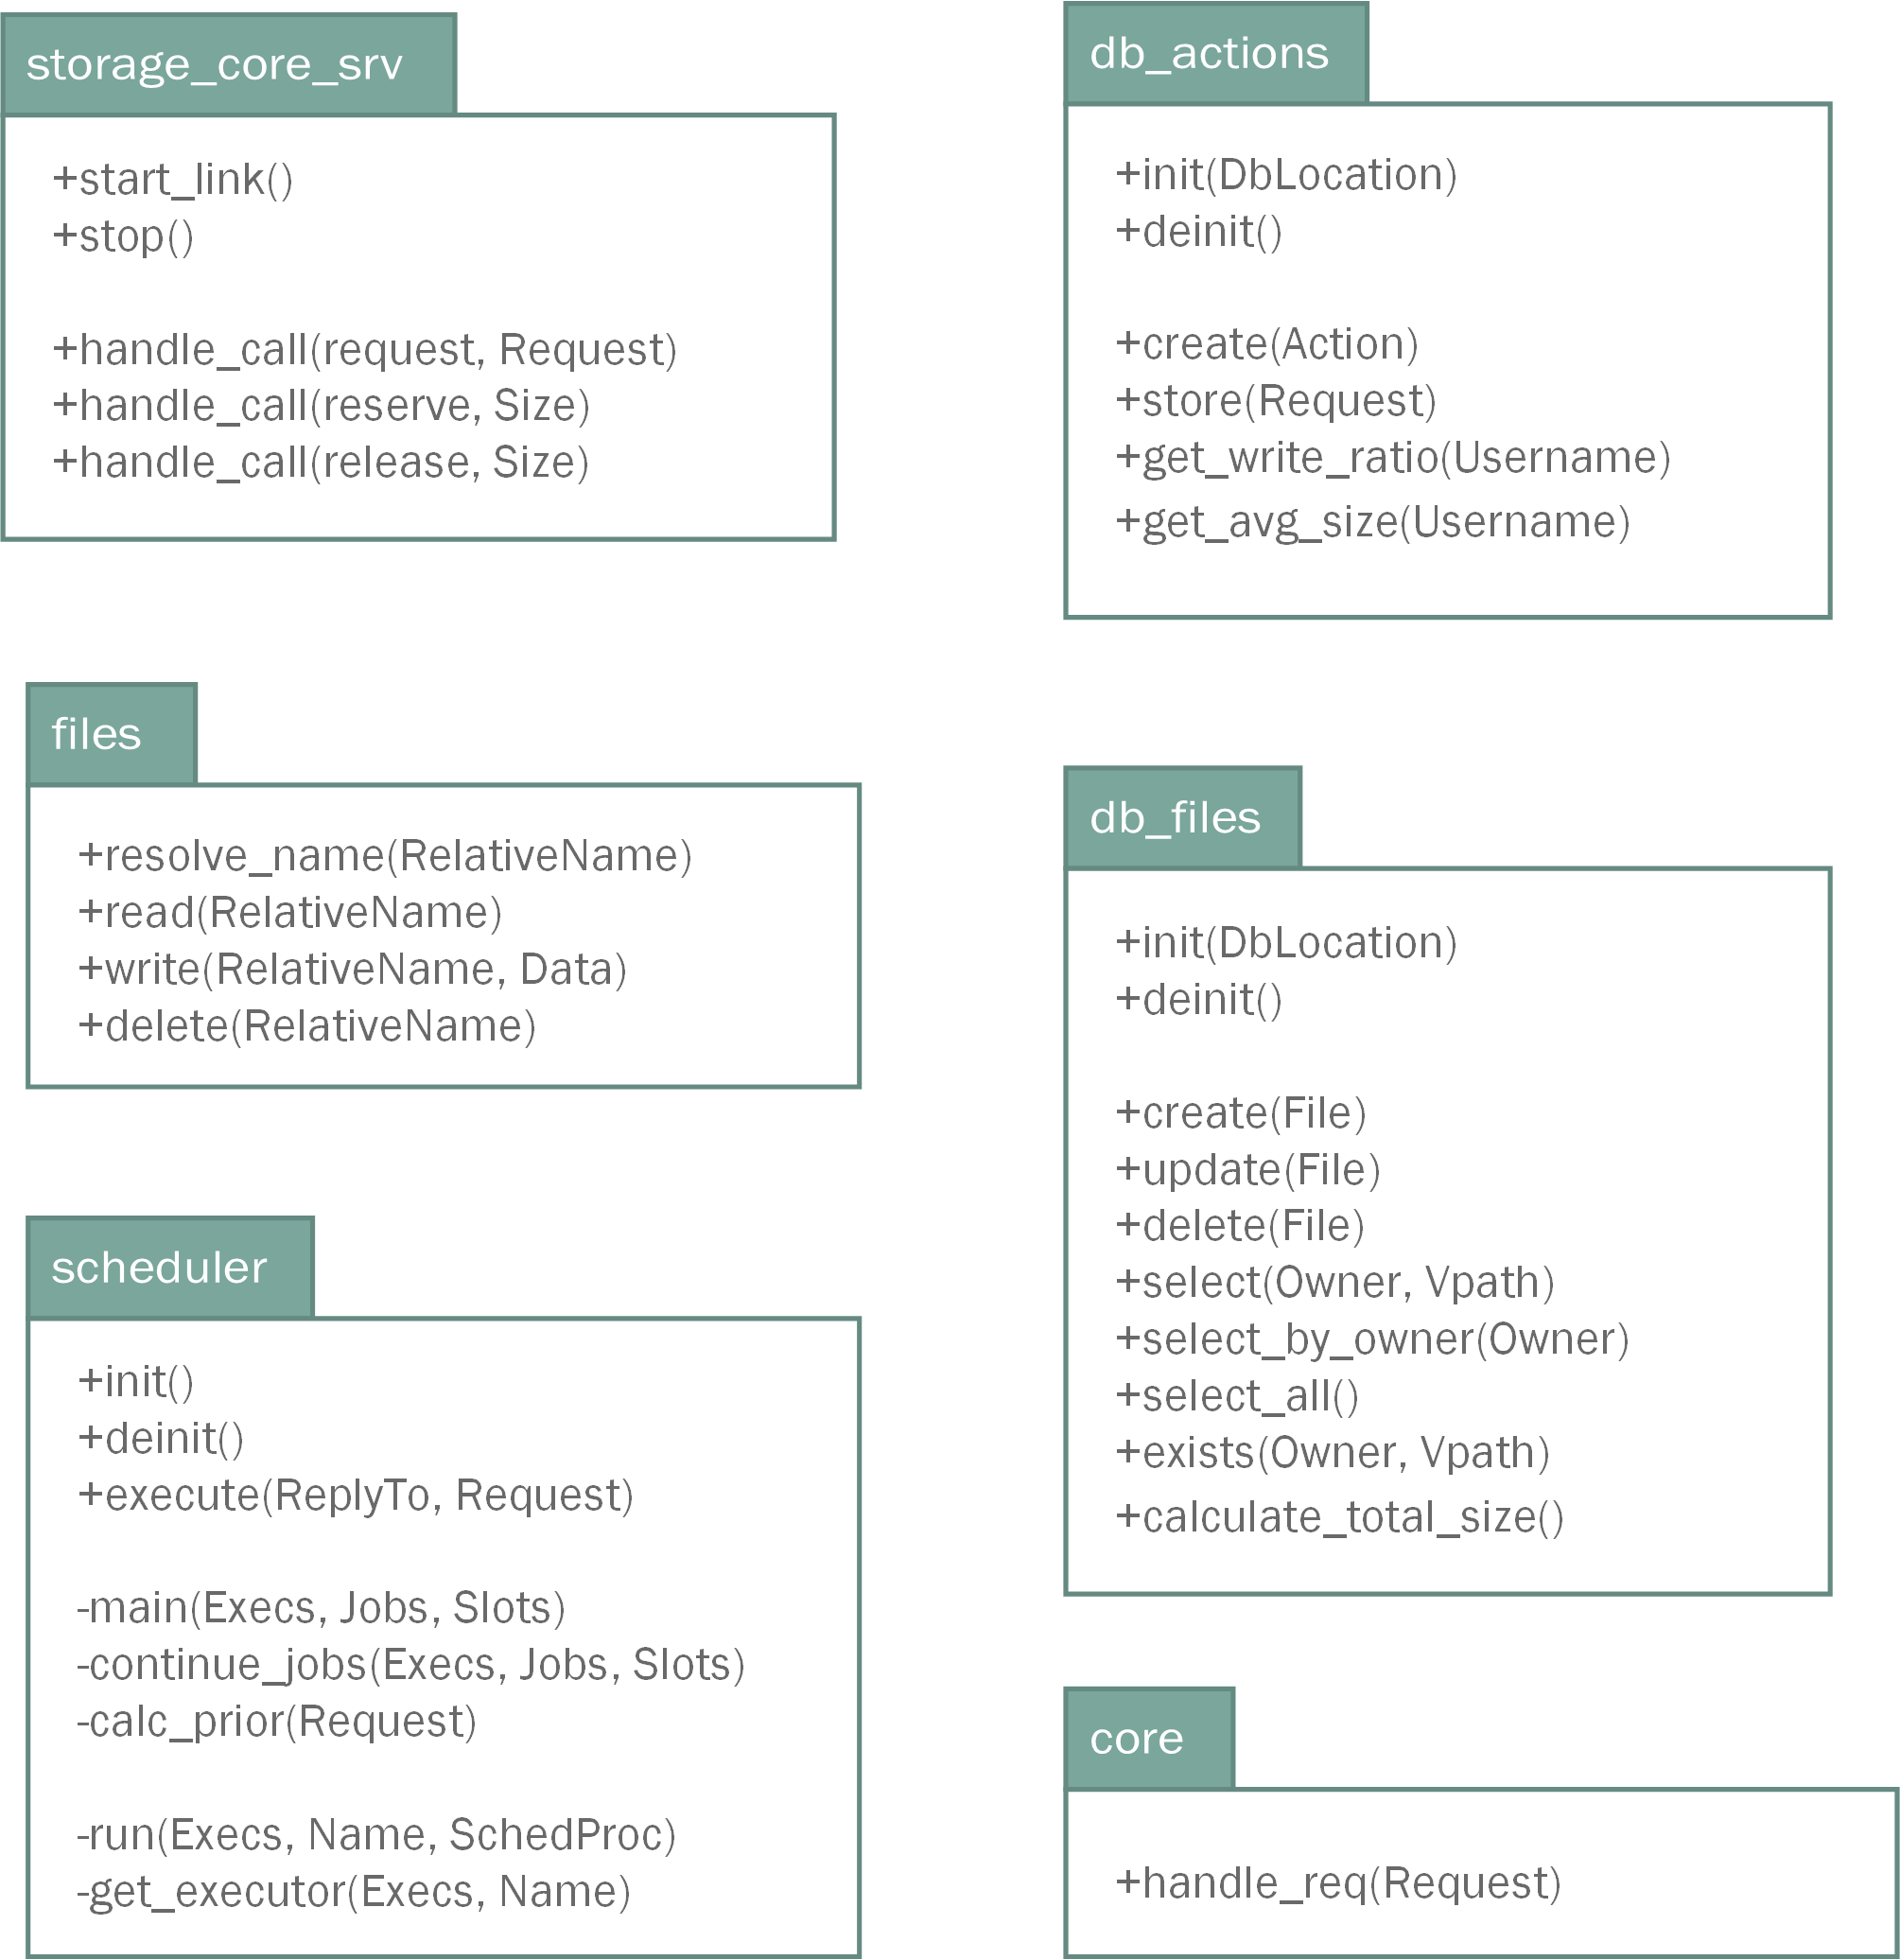
\includegraphics[width=0.9\textwidth]{core-module}
	\caption[Struktura modułu wykonawczego.]{Podmoduły składowe modułu core.}
	\label{fig:core-module}
\end{figure}

Każdy węzeł dysponuje określoną ilością miejsca na przechowywane pliki. Kiedy tworzone jest nowy plik, dostępne miejsce maleje. W punkcie 1.3.5 Moduł komunikacyjny przedstawiono zasady działania wywołań call(reserve, Size) i call(release, Size). Trzecia z funkcji gen\_servera, call(request, Request) odpowiedzialna jest za obsługę zapytania i przyjmuje w argumencie strukturę Request.
Zapytanie jest natychmiast przekazywane do modułu schedulera, który wyszukuje odpowiedni wątek wykonawczy i przekazuje mu zapytanie do obsługi. Wątek ten jest również odpowiedzialny za umieszczenie w bazie informacji o wykonanej akcji.
Ogólny diagram sekwencji przedstawia \autoref{fig:core-seq-1}. Rozważany przypadek to zapytanie read. Wszystkie inne wyglądają jednak tak samo. Scheduler został ukazany jako jeden, atomowy obiekt. Dalej opisany jest w szczegółach.

\begin{figure}[!htbp]
	\centering
	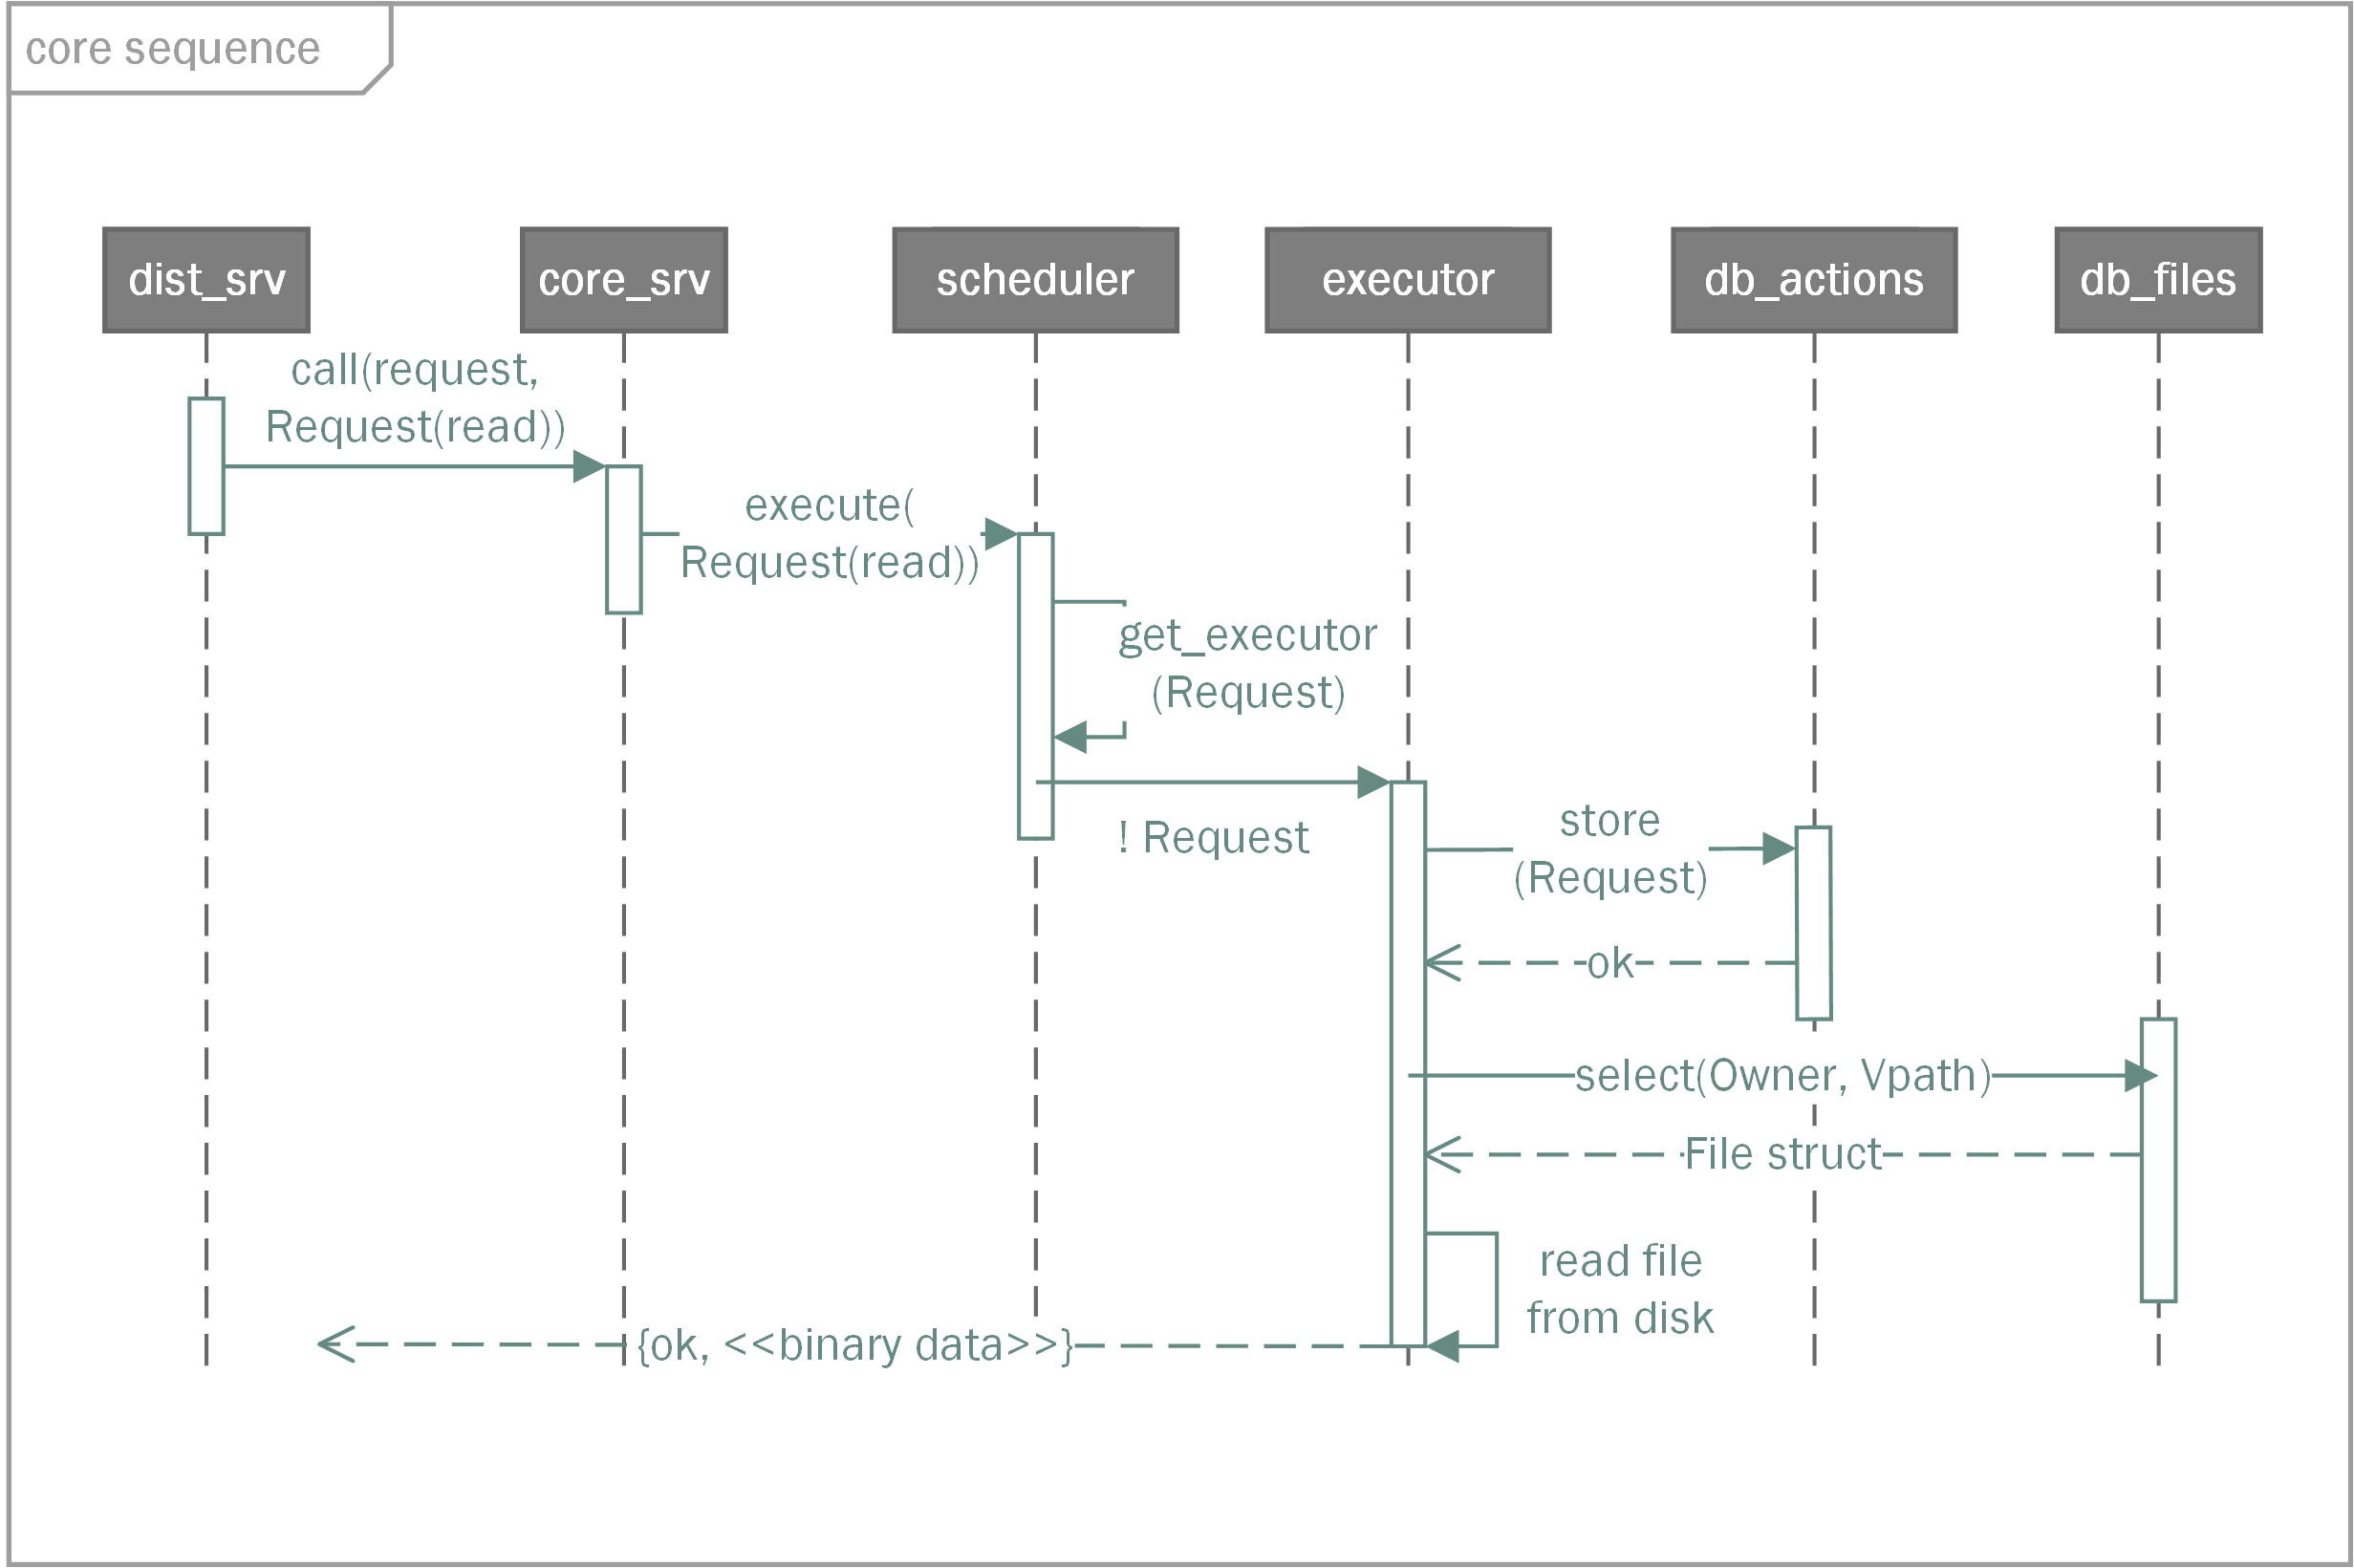
\includegraphics[width=0.9\textwidth]{core-seq-1}
	\caption{Obsługa żądania odczytu pliku w module wykonawczym.}
	\label{fig:core-seq-1}
\end{figure}

\paragraph{Scheduler} Scheduler jest modułem szeregującym zapytania trafiające do danego węzła. Zarządza on pulą wątków wykonawczych (executor), odpowiedzialnych za bezpośrednią obsługę zadań. Każdy plik (każda ścieżka) ma przydzielony jeden wątek wykonawczy. Zapytania dotyczące konkretnego pliku zawsze więc są obsługiwane przez jeden wątek. Wątek wykonawczy tworzony jest po próbie dostępu do określonego pliku i ulega zniszczeniu po określonym czasie bezczynności (domyślnie 180 sekund).

Po otrzymaniu zapytania o konkretny plik, scheduler znajduje skojarzony z nim wątek wykonawczy i umieszcza zadanie (strukturę Request) w kolejce wiadomości tego procesu (message queue języka Erlang).

Scheduler umieszcza wszystkie przychodzące akcje w kolejce priorytetowej. Zapisuje je w postaci krotek \{Priority, Executor\}, gdzie Priority to priorytet obliczony dla danego zapytania natomiast Executor to identyfikator wątku wykonawczego gdzie trafiło to zapytanie.

Przed rozpoczęciem przetwarzania kolejnego zadania, wątek wykonawczy czeka na pozwolenie od schedulera. Po każdym zakończonym zadaniu informuje scheduler o zakończeniu jego obsługi.

Scheduler uruchamia N (domyślnie 4) pierwszych wątków wykonawczych z kolejki priorytetowej. Jeżeli jakiś wątek skończy przetwarzać jakieś zapytanie, scheduler wybiera z kolejki w jego miejsce wątek o najwyższym priorytecie.

\begin{figure}[!htbp]
	\centering
	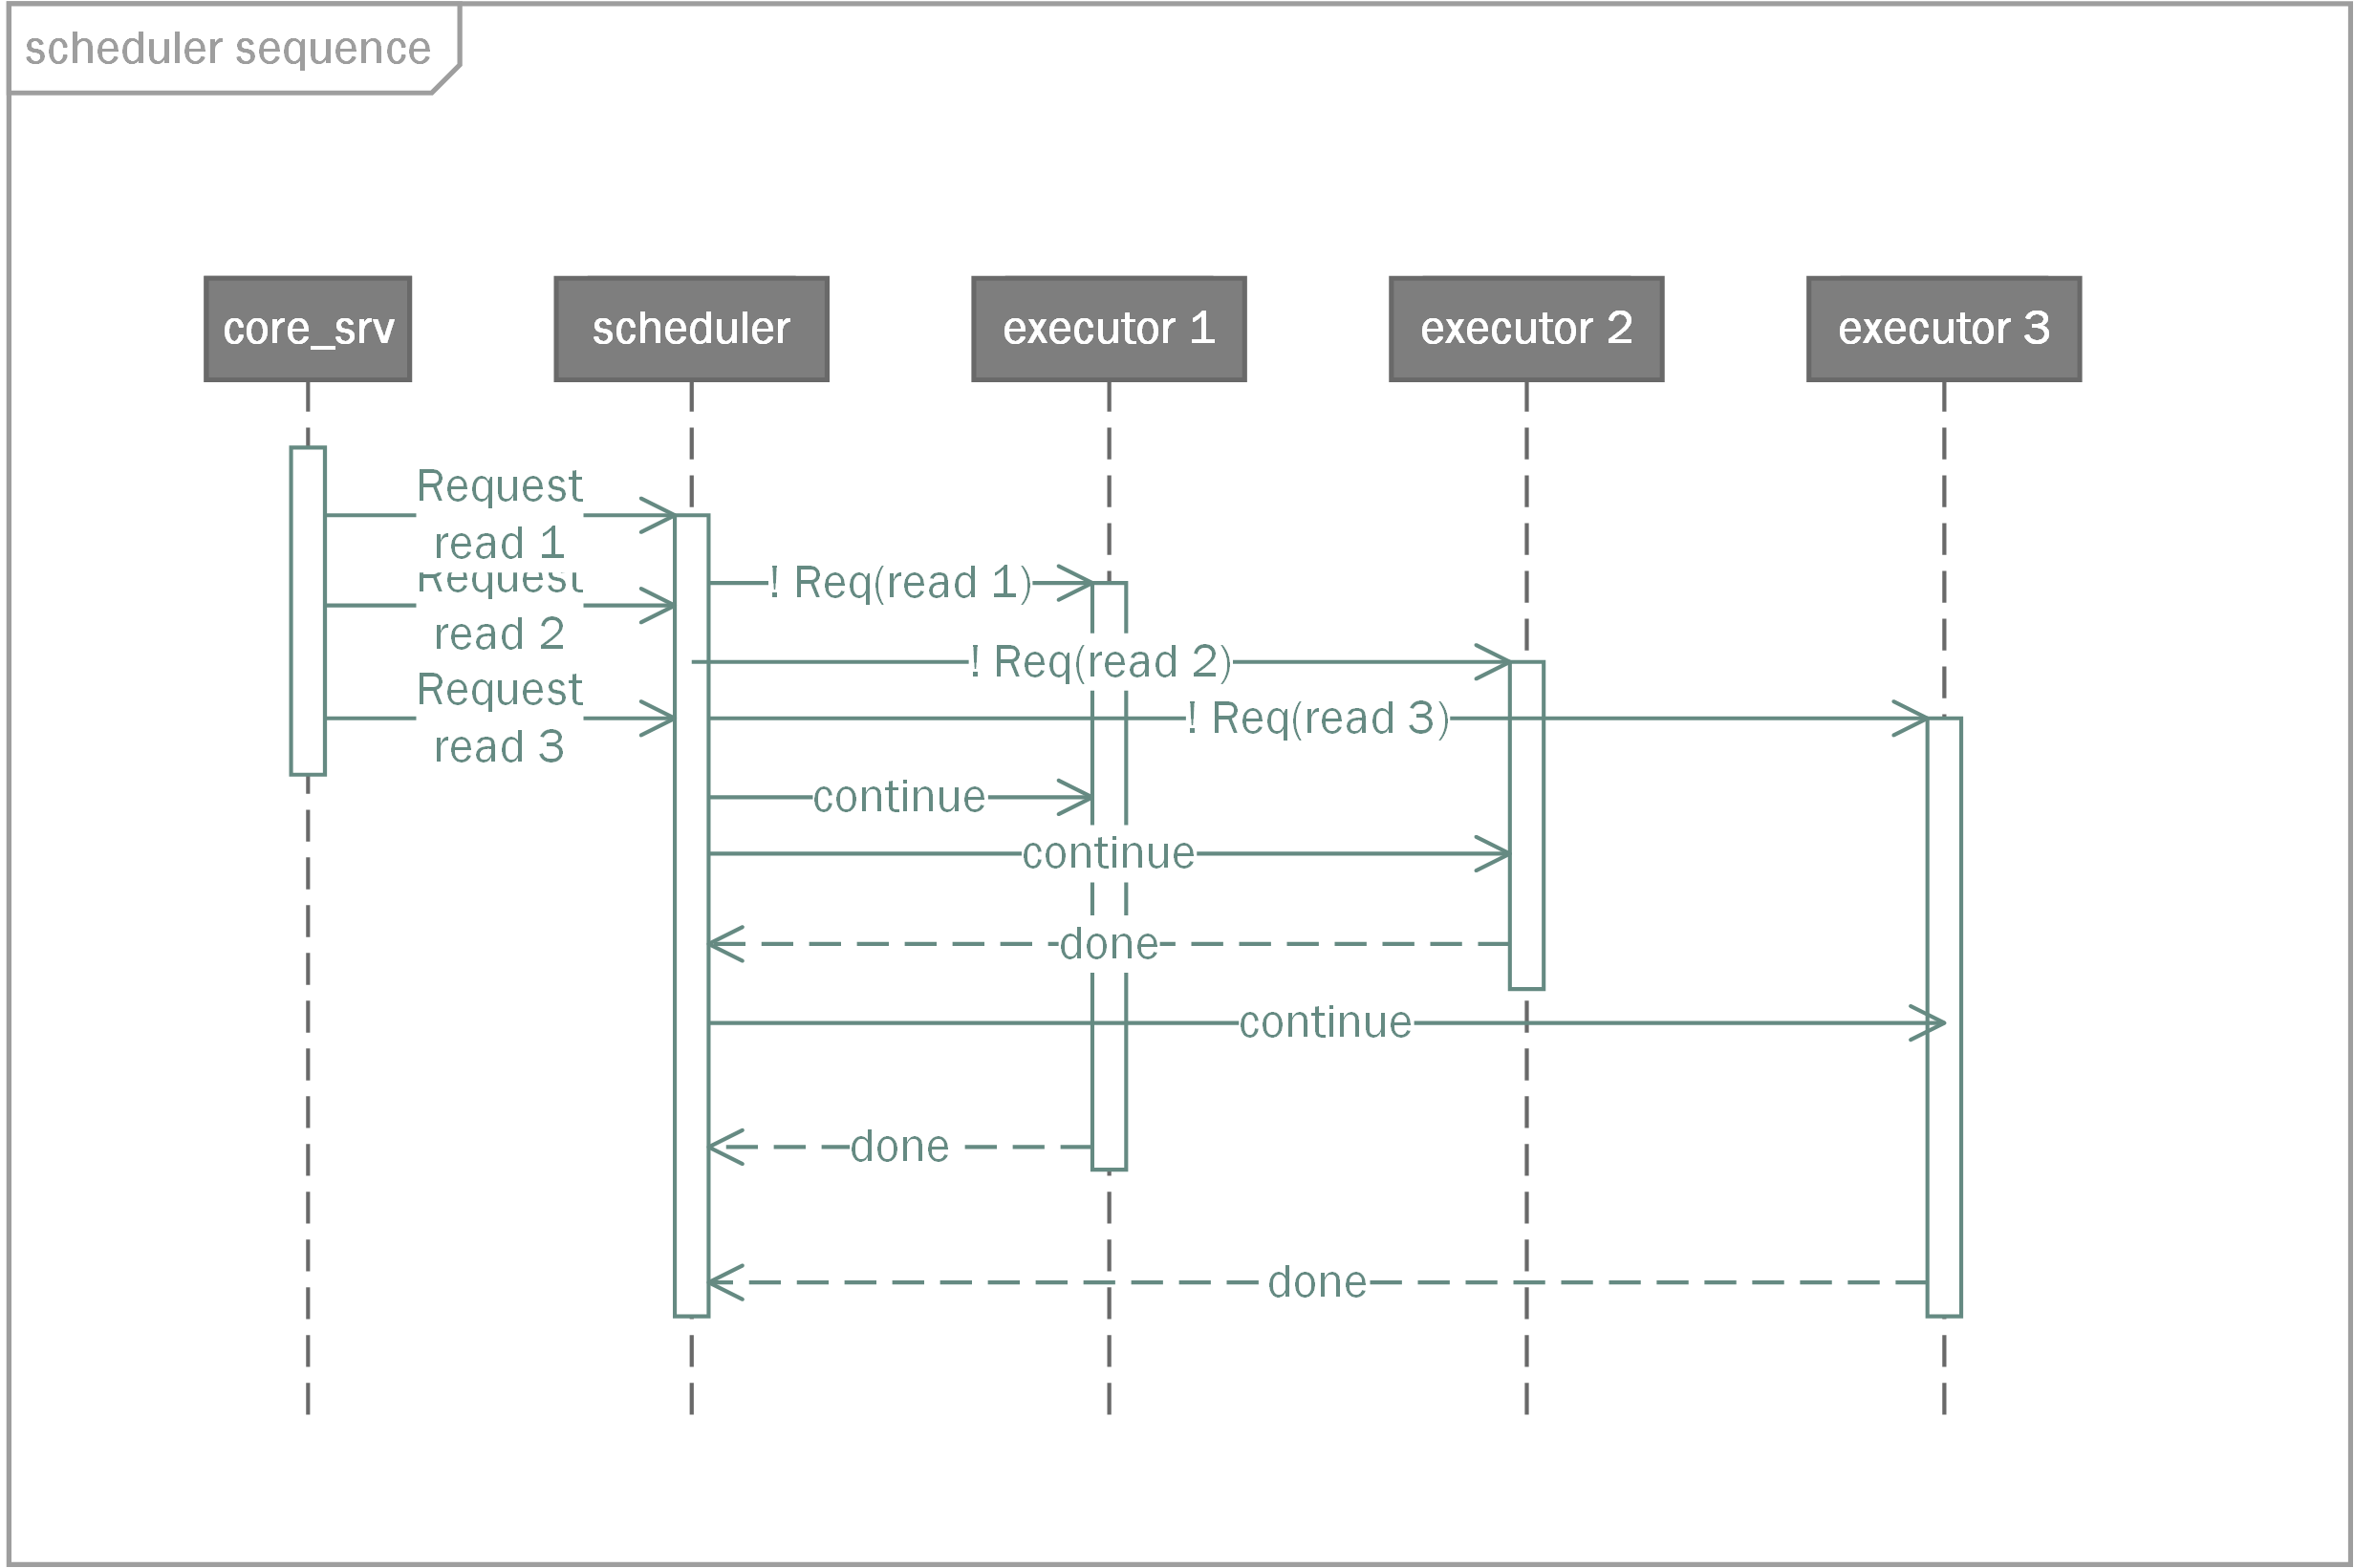
\includegraphics[width=0.9\textwidth]{core-seq-2}
	\caption[Sekwencja uruchamiania wątków wykonawczych.]{Sekwencja uruchamiania wątków wykonawczych (maksymalnie dwa jednoczesne wątki). Pojawiają się trzy zapytania o trzy różne pliki. Każde z nich trafi zatem do innego wątku wykonawczego. Zadania są kolejkowane w wątkach zgodnie z kolejnością przybycia (kolejność w obrębie jednego wątku wykonawczego musi zostać zachowana). Wątki nie rozpoczynają pracy od razu – scheduler wysyła do każdego z nich komunikat continue. Dwa wątki zostały uruchomione jednocześnie. Trzeci czekał na zakończenie pracy przez jeden z nich.}
	\label{fig:core-seq-2}
\end{figure}
